\documentclass[a4paper,10pt,oneside]{book} 
\usepackage{CS_report}
\usepackage[T1]{fontenc}   

\makeatletter
\pretocmd{\tableofcontents}{\hypersetup{linkcolor=black}}{}{}
\makeatother
\captionsetup[figure]{margin=1.5cm,font=small,name={Gambar},labelsep=colon}
\captionsetup[table]{margin=1.5cm,font=small,name={Tabel},labelsep=colon}

\begin{document}

    \frontmatter
    
    \begin{titlepage}
        \begin{center}
            
            \vspace{5cm}
            {\LARGE \textbf{Laporan Tugas Kecil 1}}\\[0.5cm]
            {\Large IF2211 \textsc{Strategi Algoritma}}\\[0.2cm]
            {\large Penyelesaian Permainan Queens Linkedin}\\[0.2cm]
            {\normalsize Semester II Tahun 2025/2026}\\[1.5cm]

            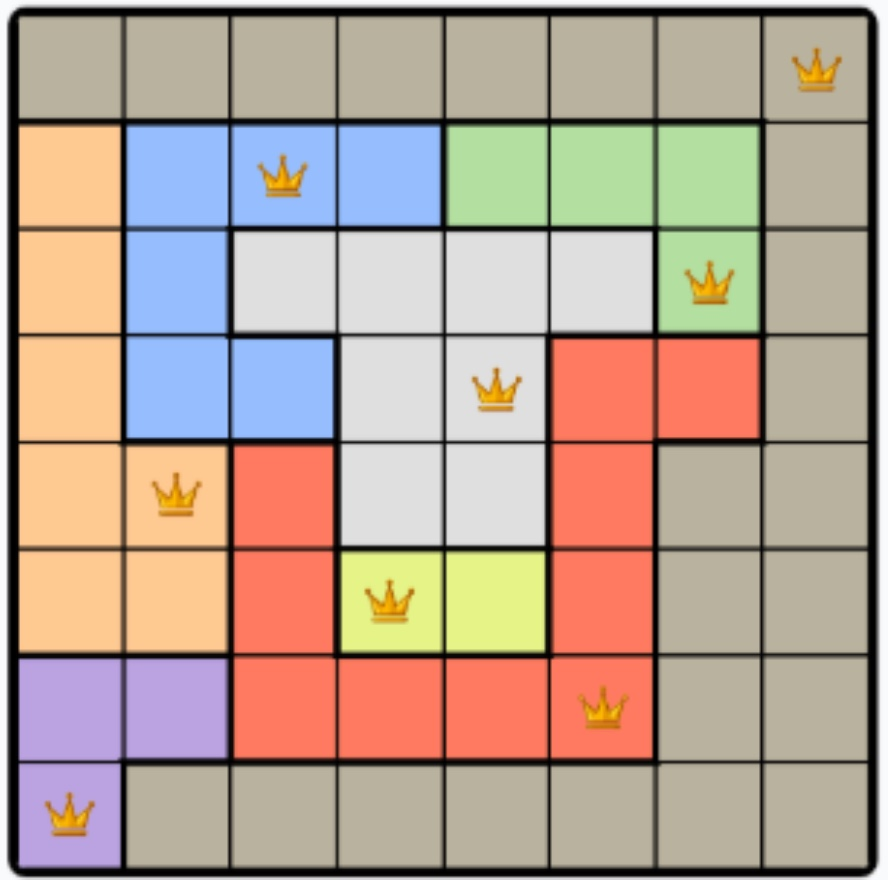
\includegraphics[width=14cm]{img/cover.png}\\[2cm]
            
            \Large{Jonathan Kris Wicaksono}\\
            \Large{13524023}\\
            \vspace{2cm}

            {\normalsize 
            Laboratorium Ilmu dan Rekayasa Komputasi\\
            Program Studi Teknik Informatika\\
            Sekolah Teknik Elektro dan Informatika\\
            Institut Teknologi Bandung}\\[0.3cm]
    
        \end{center}
    \end{titlepage}
    
    \tableofcontents
    \listoftables
    \listoffigures
    
    \mainmatter
    \chapter{Implementasi Algoritma}

Dalam permainan Queens LinkedIn, tujuannya adalah menempatkan satu \textit{queen} pada setiap baris di papan berukuran $N \times M$ yang terbagi menjadi daerah warna, dengan syarat: tepat satu queen pada setiap baris, kolom, dan daerah warna, serta tidak boleh ada dua queen yang saling bersebelahan (termasuk diagonal). Program ini ditulis dalam bahasa C++ dengan GUI menggunakan library SFML 3.0 dan mengimplementasikan algoritma Brute Force.

\section{Algoritma Brute Force}

Algoritma \textit{brute force} yang diimplementasikan bersifat murni, yaitu mengenumerasi seluruh kemungkinan penempatan queen tanpa heuristik apapun.

Berikut adalah langkah-langkah detail dari algoritma brute force yang diimplementasikan pada fungsi \texttt{solve\_bf()}:

\begin{enumerate}
    \item Program menerima masukan berupa \textit{grid} berukuran $N \times M$ yang dibaca dari file \texttt{.txt}. Setiap huruf pada grid merepresentasikan daerah warna.
    \item Dibuat sebuah \textit{array} \texttt{curr} berukuran $N$, diinisialisasi dengan $[0, 0, \dots, 0]$. Elemen \texttt{curr[i]} menyatakan kolom tempat queen diletakkan pada baris ke-$i$.
    \item Untuk setiap konfigurasi \texttt{curr}, dilakukan validasi terhadap seluruh syarat permainan:
    \begin{itemize}
        \item \textbf{Syarat kolom}: Tidak boleh ada dua queen pada kolom yang sama, diperiksa dengan membandingkan \texttt{curr[i]} terhadap \texttt{curr[prev]} untuk seluruh baris sebelumnya.
        \item \textbf{Syarat warna}: Tidak boleh ada dua queen pada daerah warna yang sama, diperiksa dengan membandingkan \texttt{grid[i][curr[i]]} terhadap \texttt{grid[prev][curr[prev]]}.
        \item \textbf{Syarat adjacency}: Queen pada baris berurutan tidak boleh berada pada kolom yang bersebelahan, diperiksa dengan kondisi $|curr[i] - curr[i-1]| \leq 1$.
    \end{itemize}
    \item Jika seluruh syarat terpenuhi, konfigurasi disimpan sebagai solusi.
    \item Jika tidak valid, konfigurasi di-\textit{increment}: \texttt{curr[N-1]} dinaikkan 1; jika melebihi $M$, di-\textit{reset} ke 0 dan \texttt{curr[N-2]} dinaikkan, dan seterusnya.
    \item Proses berulang hingga solusi ditemukan atau seluruh $M^N$ konfigurasi habis diperiksa.
\end{enumerate}

Algoritma ini memiliki kompleksitas waktu \textbf{$O(M^N \cdot N)$} karena setiap konfigurasi memerlukan $O(N)$ untuk validasi.

\begin{algorithm}[H]
\caption{Algoritma Brute Force Queens}
\begin{algorithmic}[1]
\Procedure{SolveBruteForce}{$grid, N, M$}
    \State $curr \gets [0, 0, \dots, 0]$ \Comment{Array berukuran $N$}
    \While{\textbf{true}}
        \State $iter \gets iter + 1$
        \State $valid \gets$ \textbf{true}
        \For{$i \gets 0$ \textbf{to} $N-1$}
            \State $c \gets curr[i]$
            \If{$c \geq M$} $valid \gets$ \textbf{false}; \textbf{break} \EndIf
            \For{$prev \gets 0$ \textbf{to} $i-1$}
                \If{$curr[prev] = c$} $valid \gets$ \textbf{false}; \textbf{break} \EndIf \Comment{Kolom sama}
                \If{$grid[prev][curr[prev]] = grid[i][c]$} $valid \gets$ \textbf{false}; \textbf{break} \EndIf \Comment{Warna sama}
            \EndFor
            \If{$i > 0$ \textbf{and} $|c - curr[i-1]| \leq 1$} $valid \gets$ \textbf{false}; \textbf{break} \EndIf \Comment{Adjacency}
        \EndFor
        \If{$valid$} \Return $curr$ \Comment{Solusi ditemukan}
        \EndIf
        \State \Comment{Increment ke konfigurasi berikutnya}
        \State $idx \gets N - 1$
        \While{$idx \geq 0$}
            \State $curr[idx] \gets curr[idx] + 1$
            \If{$curr[idx] < M$} \textbf{break} \EndIf
            \State $curr[idx] \gets 0$; $idx \gets idx - 1$
        \EndWhile
        \If{$idx < 0$} \Return \texttt{None} \Comment{Tidak ada solusi}
        \EndIf
    \EndWhile
\EndProcedure
\end{algorithmic}
\end{algorithm}

\section{Fitur Tambahan Program}

Selain algoritma pencarian, program juga mengimplementasikan:

\begin{enumerate}
    \item \textbf{GUI (SFML 3.0)}: Panel kontrol dengan tombol-tombol interaktif (BROWSE, LOAD, SOLVE, STOP, SAVE TXT, SAVE IMG), pemilihan algoritma, dan slider kecepatan visualisasi.
    \item \textbf{Live Visualization}: Setiap iterasi pencarian divisualisasikan secara \textit{real-time} pada papan GUI. Kecepatan dapat diatur melalui slider (TURBO / FAST / SLOW).
    \item \textbf{Validasi Input}: Program memverifikasi:
    \begin{itemize}
        \item Seluruh baris memiliki panjang yang sama
        \item Karakter hanya boleh berupa huruf A--Z
        \item Jumlah region warna unik harus sama dengan jumlah baris ($N$)
    \end{itemize}
    \item \textbf{Output as Text}: Solusi dapat disimpan sebagai file \texttt{.txt} melalui tombol SAVE TXT, lengkap dengan waktu pencarian dan jumlah iterasi.
    \item \textbf{Output as Image}: Solusi dapat disimpan sebagai file PNG melalui tombol SAVE IMG.
\end{enumerate}

    \input{chapters/02_Source Code}
    \chapter{Pengujian}
Program yang dibuat dapat menyelesaikan papan Queens LinkedIn dengan masukan berupa file \texttt{.txt} melalui antarmuka GUI berbasis SFML. Berikut adalah hasil pengujian menggunakan 5 test case yang berbeda, beserta penanganan input tidak valid.

\section{Test 1: Papan berukuran $9\times 9$ (in1.txt)}
\begin{table}[H]
    \centering
    \begin{minipage}{0.45\textwidth}
        \centering
        \captionof{table}{Input Test 1}
        \renewcommand{\arraystretch}{1.2}
        \setlength{\tabcolsep}{40pt}
        \begin{tabular}{|l|}
            \hline
            \phantom{text}\\
            AAABBCCCD\\
            ABBBBCECD\\
            ABBBDCECD\\
            AAABDCCCD\\
            BBBBDDDDD\\
            FGGGDDHDD\\
            FGIGDDHDD\\
            FGIGDDHDD\\
            FGGGDDHHH\\
            \phantom{text}\\
            \hline
        \end{tabular}
    \end{minipage}
\end{table}

Program menyediakan dua format output: file teks (.txt) dan gambar (.png). Output teks berisi papan dengan posisi queen ditandai \texttt{\#}, waktu pencarian, dan jumlah iterasi. Output gambar menampilkan visualisasi GUI.

\subsection*{Output sebagai File TXT}
\begin{lstlisting}[basicstyle=\ttfamily\small]
AAABBCC#D
ABBB#CECD
ABBBDC#CD
A#ABDCCCD
BBBBD#DDD
FGG#DDHDD
#GIGDDHDD
FG#GDDHDD
FGGGDDHH#

Waktu pencarian: 1461 ms
Banyak kasus yang ditinjau: 323741637 kasus
\end{lstlisting}

\subsection*{Output sebagai Gambar (PNG)}
\begin{figure}[H]
    \centering
    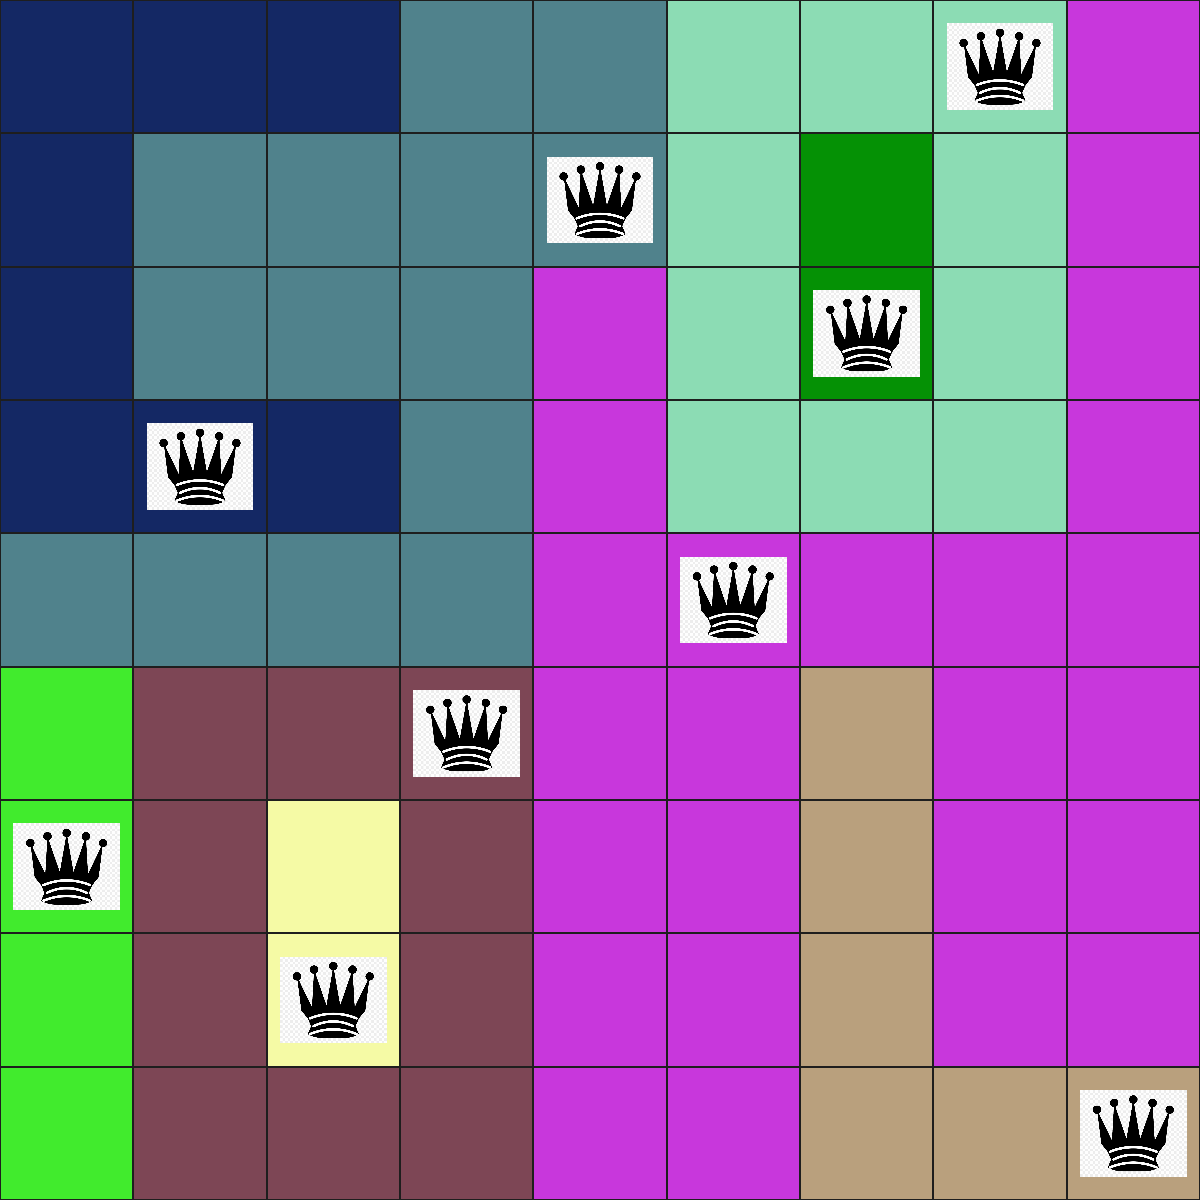
\includegraphics[width=10cm]{figures/out1.png}
    \caption{Output GUI --- Test 1}
\end{figure}

\section{Test 2: Papan berukuran $11\times 11$ (in2.txt)}

Test case ini menggunakan papan berukuran $11\times 11$ dimana setiap baris merupakan satu region warna. 

\begin{table}[H]
    \centering
    \captionof{table}{Input Test 2}
    \renewcommand{\arraystretch}{1.2}
    \setlength{\tabcolsep}{20pt}
    \begin{tabular}{|l|}
        \hline
        \phantom{text}\\
        AAAAAAAAAAA\\
        BBBBBBBBBBB\\
        CCCCCCCCCCC\\
        DDDDDDDDDDD\\
        EEEEEEEEEEE\\
        FFFFFFFFFFF\\
        GGGGGGGGGGG\\
        HHHHHHHHHHH\\
        IIIIIIIIIII\\
        JJJJJJJJJJJ\\
        KKKKKKKKKKK\\
        \phantom{text}\\
        \hline
    \end{tabular}
\end{table}

Setiap baris terdiri dari satu huruf yang sama (11 kolom), sehingga setiap baris adalah satu region warna.

Program menyediakan dua format output: file teks (.txt) dan gambar (.png).

\subsection*{Output sebagai File TXT}
\begin{lstlisting}[basicstyle=\ttfamily\small]
#AAAAAAAAAA
BB#BBBBBBBB
CCCC#CCCCCC
D#DDDDDDDDD
EEE#EEEEEEE
FFFFF#FFFFF
GGGGGGG#GGG
HHHHHHHHH#H
IIIIII#IIII
JJJJJJJJ#JJ
KKKKKKKKKK#

Waktu pencarian: 17135 ms
Banyak kasus yang ditinjau: 5599053306 kasus
\end{lstlisting}

\subsection*{Output sebagai Gambar (PNG)}
\begin{figure}[H]
    \centering
    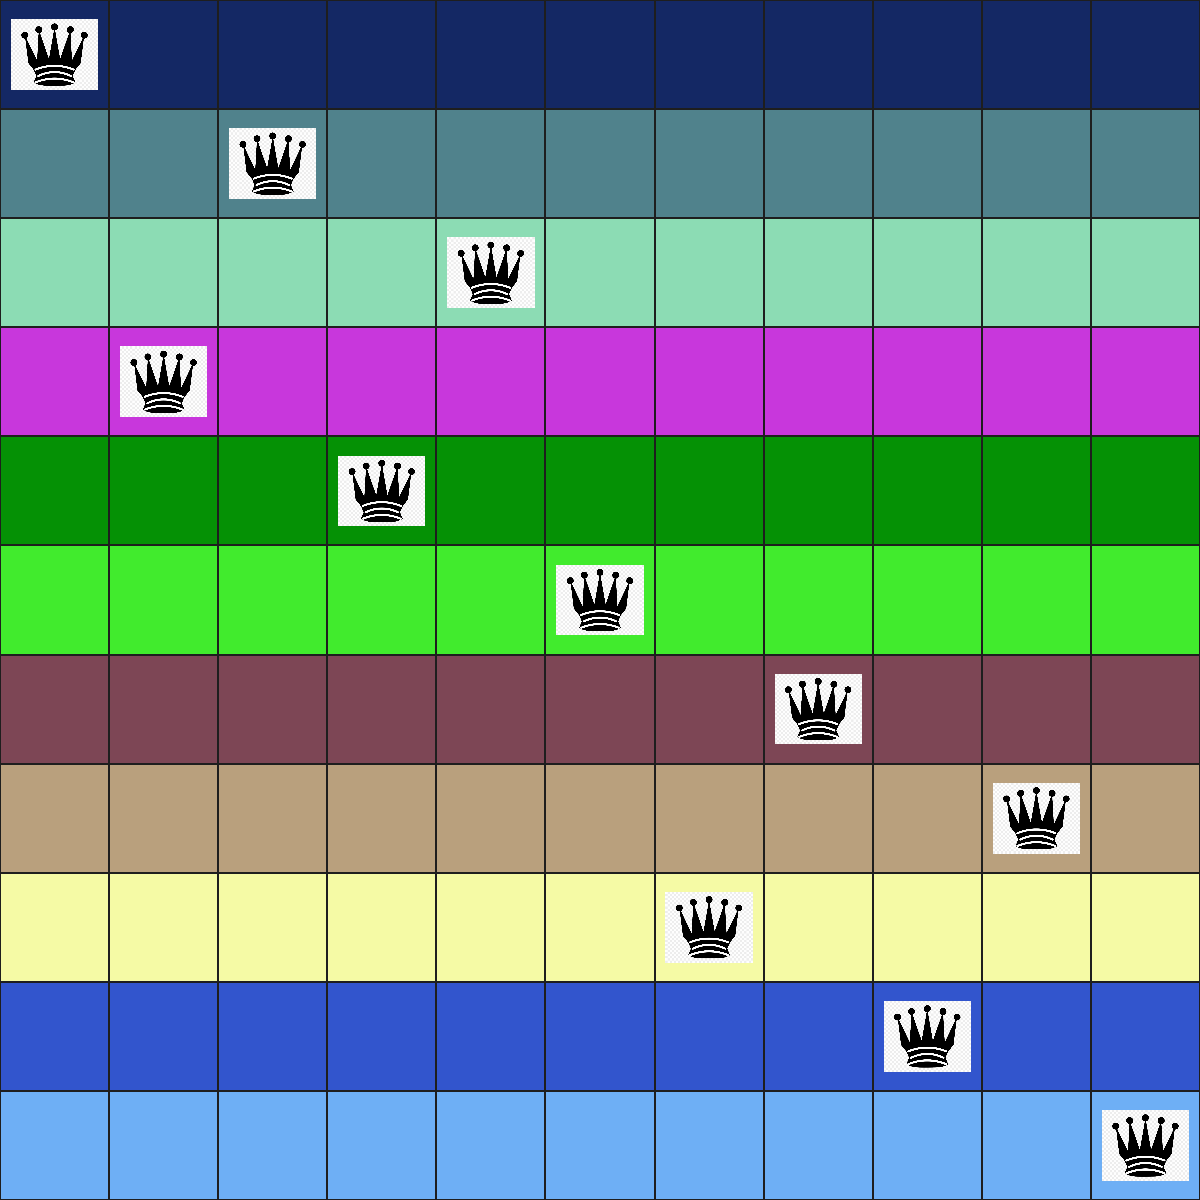
\includegraphics[width=10cm]{figures/out2.png}
    \caption{Output GUI --- Test 2}
\end{figure}

\section{Test 3: Papan berukuran $1\times 1$ (in3.txt)}

\begin{table}[H]
    \centering
    \begin{minipage}{0.45\textwidth}
        \centering
        \captionof{table}{Input Test 3}
        \renewcommand{\arraystretch}{1.2}
        \setlength{\tabcolsep}{40pt}
        \begin{tabular}{|l|}
            \hline
            \phantom{text}\\
            A\\
            \phantom{text}\\
            \hline
        \end{tabular}
    \end{minipage}
\end{table}

Papan berukuran $1\times 1$ dengan satu region. Queen langsung ditempatkan pada satu-satunya sel.

Program menyediakan dua format output: file teks (.txt) dan gambar (.png).

\subsection*{Output sebagai File TXT}
\begin{lstlisting}[basicstyle=\ttfamily\small]
#

Waktu pencarian: 0 ms
Banyak kasus yang ditinjau: 1 kasus
\end{lstlisting}

\subsection*{Output sebagai Gambar (PNG)}
\begin{figure}[H]
    \centering
    
\includegraphics[width=10cm]{figures/out3.png}
    \caption{Output GUI --- Test 3}
\end{figure}

\section{Test 4: Papan berukuran $9\times 9$ --- Tidak Ada Solusi (in4.txt)}

\begin{table}[H]
    \centering
    \begin{minipage}{0.45\textwidth}
        \centering
        \captionof{table}{Input Test 4}
        \renewcommand{\arraystretch}{1.2}
        \setlength{\tabcolsep}{40pt}
        \begin{tabular}{|l|}
            \hline
            \phantom{text}\\
            ABCDEFGHI\\
            BBCDEFGHI\\
            CCCDDEFGH\\
            DDDDDDEGH\\
            EEEEEFGHH\\
            FFFFFFGHH\\
            GGGGGGGHH\\
            HHHHHHHII\\
            IIIIIIIII\\
            \phantom{text}\\
            \hline
        \end{tabular}
    \end{minipage}
\end{table}

Karena papan ini tidak memiliki solusi yang valid (region tidak memungkinkan penempatan queen yang memenuhi semua aturan), program tidak menghasilkan file solusi .txt.

\subsection*{Output sebagai Gambar (PNG)}
\begin{figure}[H]
    \centering
    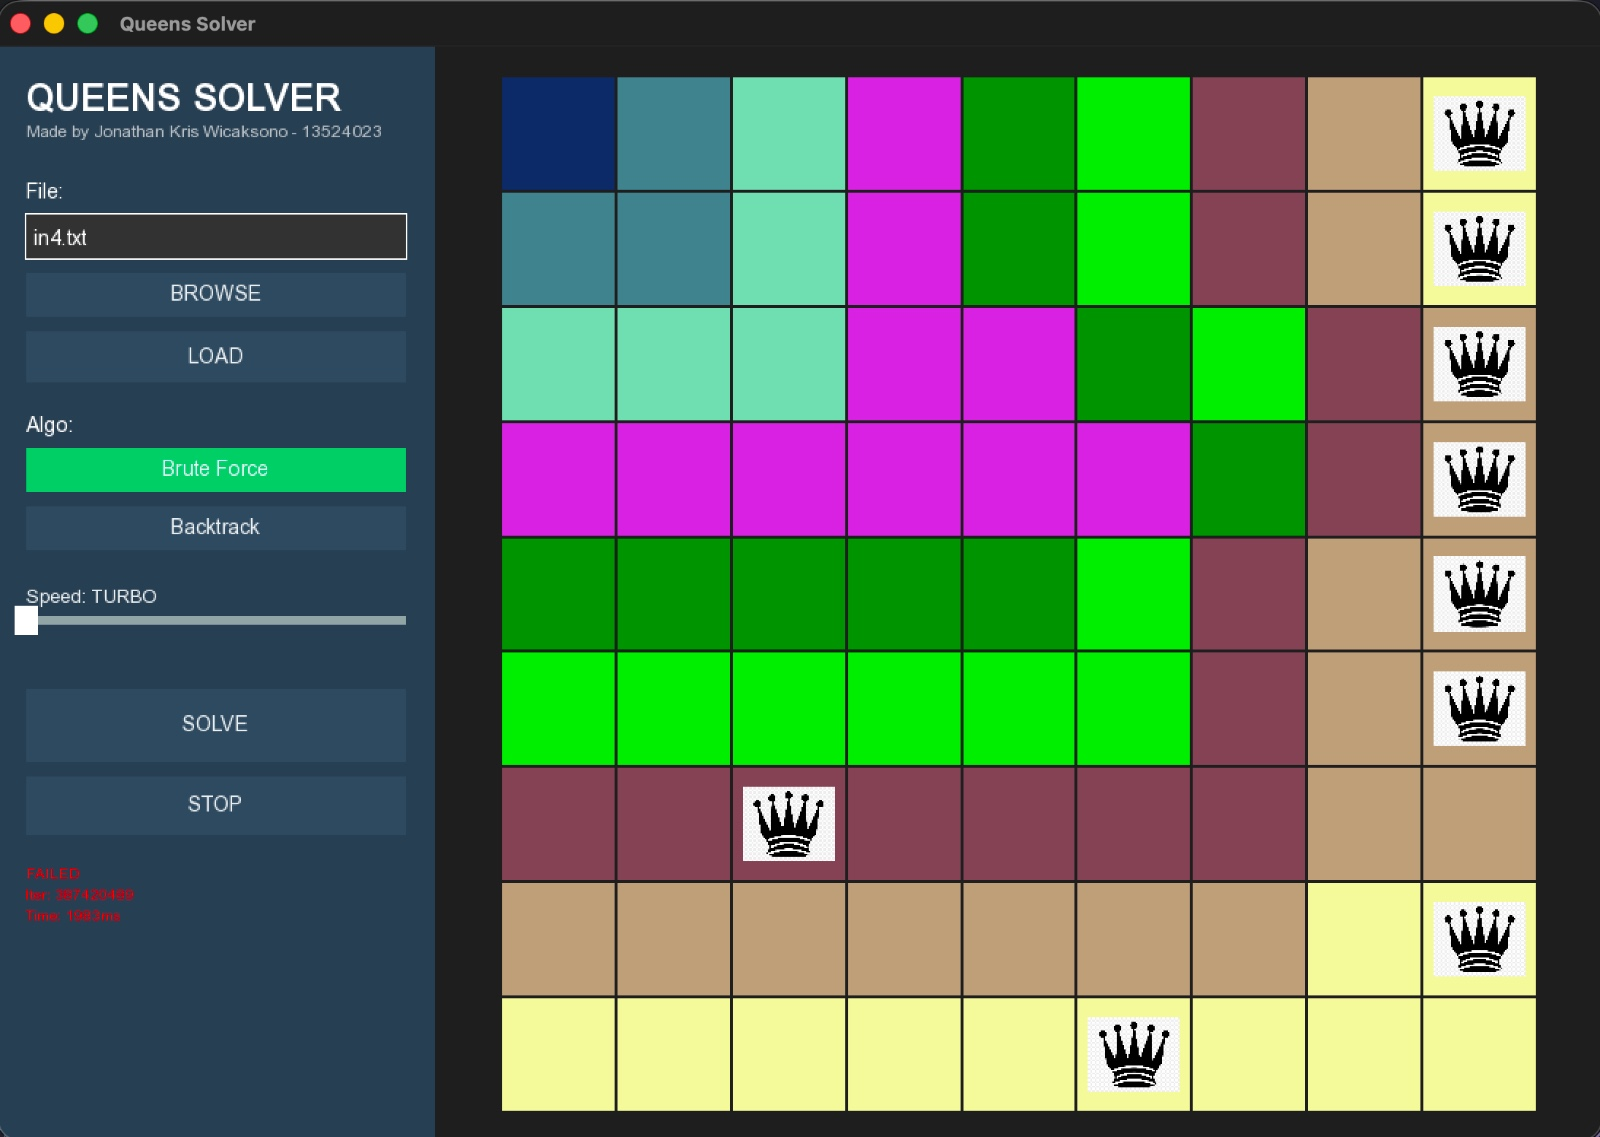
\includegraphics[width=10cm]{figures/out4.png}
    \caption{Output GUI --- Test 4 (Tidak Ada Solusi)}
\end{figure}

\section{Test 5: Input Tidak Valid --- Panjang Baris Berbeda (in5.txt)}

\begin{table}[H]
    \centering
    \begin{minipage}{0.45\textwidth}
        \centering
        \captionof{table}{Input Test 5}
        \renewcommand{\arraystretch}{1.2}
        \setlength{\tabcolsep}{30pt}
        \begin{tabular}{|l|}
            \hline
            \phantom{text}\\
            ABCDEFGHIJJ\\
            BBCDEFGHI\\
            CCCDDEFGH\\
            DDDDDDEGH\\
            EEEEEFGHH\\
            FFFFFFGHH\\
            GGGGGGGHH\\
            HHHHHHHII\\
            IIIIIIIII\\
            \phantom{text}\\
            \hline
        \end{tabular}
    \end{minipage}
\end{table}

Program berhasil mendeteksi bahwa input tidak valid karena panjang baris tidak konsisten, dan menampilkan pesan error pada panel status GUI.

Karena input tidak valid, program tidak menghasilkan file solusi .txt. Output hanya berupa pesan error yang ditampilkan di GUI.

\subsection*{Output sebagai Gambar (PNG)}
\begin{figure}[H]
    \centering
    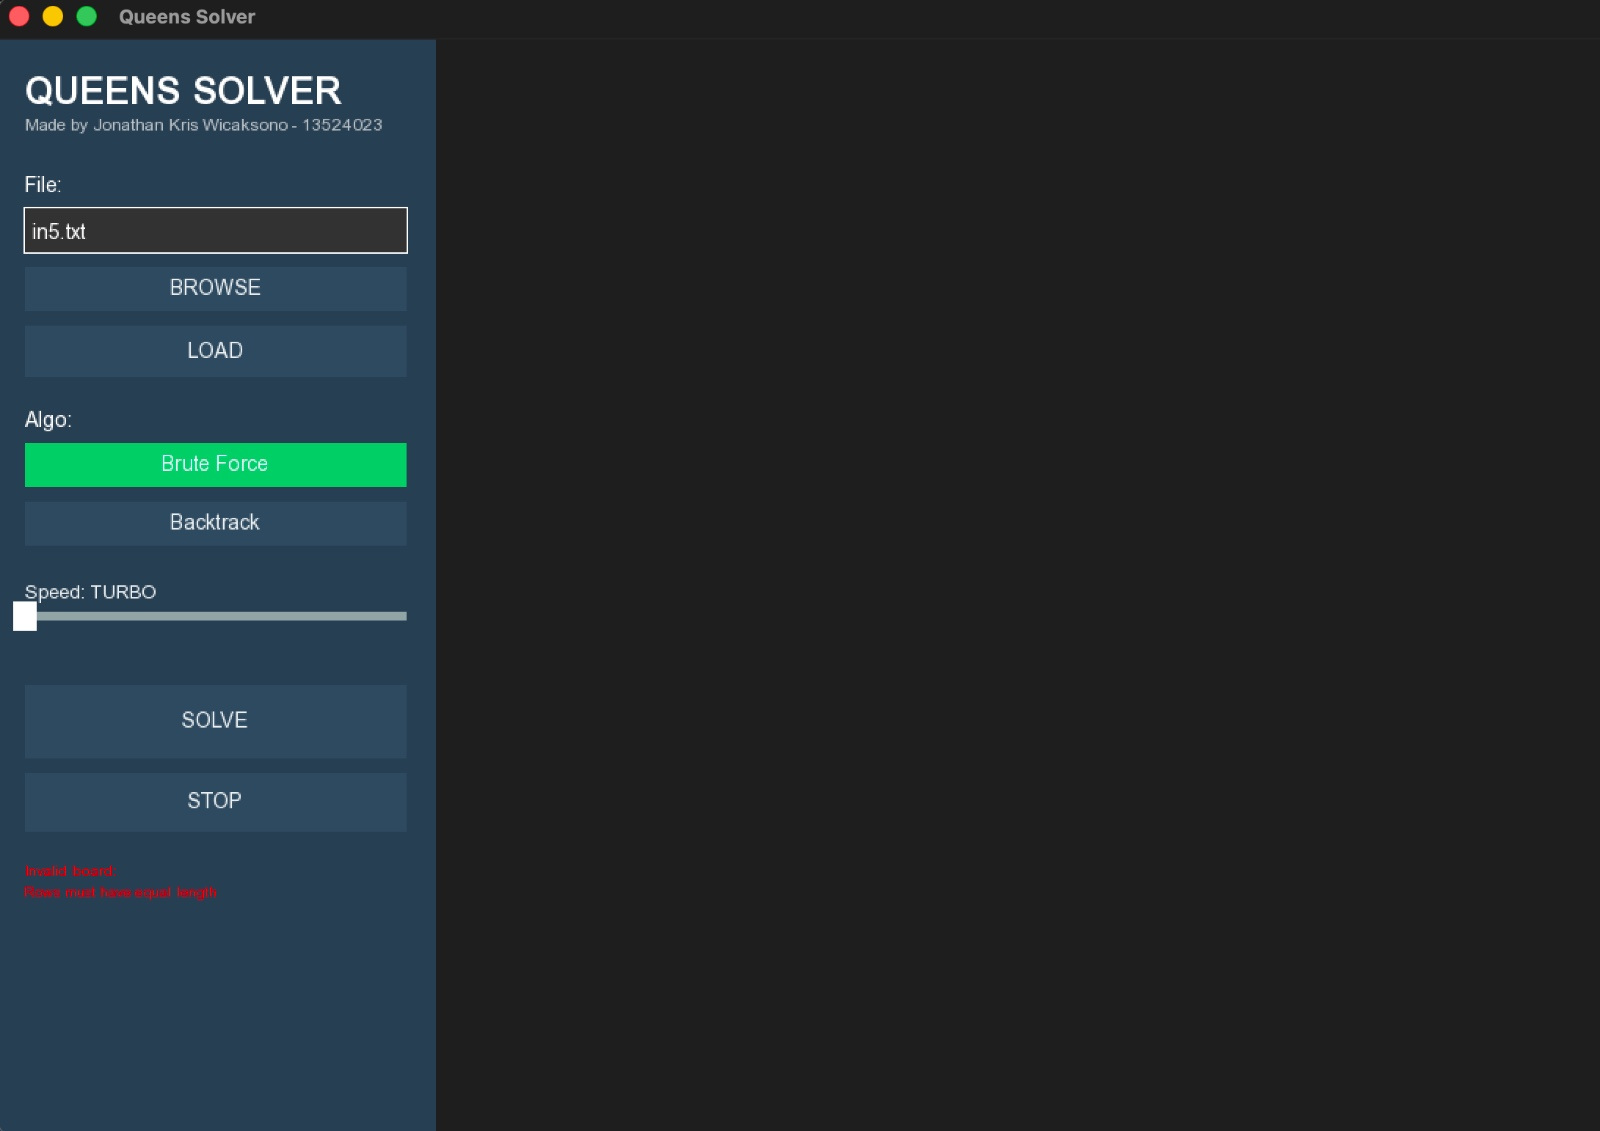
\includegraphics[width=10cm]{figures/out5.png}
    \caption{Output GUI --- Test 5 (Input Tidak Valid)}
\end{figure}

    \input{chapters/lampiran}
    Tugas ini disusun sepenuhnya tanpa bantuan kecerdasan buatan (\textit{Generative AI}),
melainkan hasil pemikiran dan analisis mandiri.
\begin{flushright}
    \begin{minipage}{0.4\textwidth}
        \centering
        \vspace{2cm}
        \rule{5cm}{0.4pt}\\
        Jonathan Kris Wicaksono [13524023]
    \end{minipage}
\end{flushright}
\end{document}
